% ==============================================================
\chapter{Introduction}
% ==============================================================

The availability of genome sequences is a key prerequisite for modern 
biological research.
After the discovery of the DNA double helix structure \citep{Watson1953},
genome sequencing have been developed over the decades, culminating in
the publication of the full human genome sequence in 2001 \citep{Venter2001}.
Aside from the ambiguities introduced by non-coding regions in the genome 
\citep{Gilbert1978} and alternative splicing of genes \citep{Black2003}, 
the genome provides, in theory, all necessary information about which proteins 
can potentially be expressed in a cell.

However, in order to study the dynamic nature of a cell or organism, as for 
example in response to changing environmental conditions, the static information
provided by the genome is not sufficient. 
For this purpose, the transcriptome provides information about gene expression
at the RNA level. 
DNA microarray techniques can be employed to screen the regulation of many
genes in parallel on the transcript level \citep{Schena1995}.

Complementing transcriptomics, the field of proteomics deals with the total
set of proteins expressed in a cell, tissue, or organism, at a defined time
point and under certain conditions \citep{Yarmush2002, Yates2009}.
In comparison to transcriptomics, proteomics is situated at the stage of 
translation of proteins and therefore most accurately reflects the current
state of the cell. 
Mass spectrometry provides an excellent means for proteome analysis
\citep{Aebersold2003}, with speed, accuracy, and sensivity rapidly increasing
within the past two decades.
The two major goals of mass spectrometry-based proteomics are protein 
identification and quantitation.
However, since most proteins are too heavy to be directly measured, the
analysis is usually performed on the peptide level, with proteins digested
prior to the measurement using proteolytic enzymes such as Trypsin, Lys-C, or 
Pepsin. 
The inherent ambiguity introduced by protein isoforms or alternative splicing
poses an additional challenge when peptide identifications are shifted to
the protein level.
In addition to the raw amino acid sequence encoded by a gene, post-translational
modifications play an important role in defining the actual function of a
protein.
Post-translational modifications may modify a protein by adding an enzyme or by
chemically modifying certain residues.
Furthermore, structural changes may result from the formation of disulfide 
bridges between two cysteine residues.
Employing mass spectrometry, it is possible not only to identify peptides and
proteins, but also to study their various modifications.
Another application of mass-spectrometry based analysis is the localization of
proteins to certain compartments of a cell, for example by semi-quantitative
analysis.

An example mass-spectrometry based proteomics workflow for peptide identification
is depicted in Fig.~\ref{fig:proteomics-overview}.

\begin{figure}
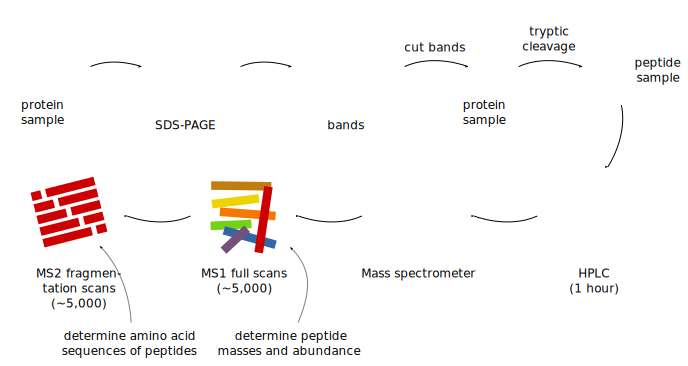
\includegraphics[width=\textwidth]{figures/Proteomics.jpg}
\caption{
{\bf Caption.} 
Caption here.
}
\label{fig:proteomics-overview}
\end{figure}

% --------------------------------------------------------------
\section{Acquisition of mass spectrometric data}
% --------------------------------------------------------------

\subsection{Preprocessing of biological samples}

\begin{todo}
SDS-PAGE, HPLC, SCX, IEF
\end{todo}

\subsection{Ionization of molecules}

\begin{todo}
ESI, MALDI
\end{todo}

\subsection{Mass analysis}

\begin{todo}
TOF, IT, Orbitrap
\end{todo}

\subsection{Mass spectra}

\begin{todo}
data formats (DTA, MGF, mzData, mzXML, mzML)
\end{todo}

\subsubsection{Full scans (MS)}

\begin{todo}
precursor peaks
\end{todo}

\begin{figure}[h]
\includegraphics[width=\textwidth]{figures/ms1-scan.jpg}
\caption{
{\bf Example of a full scan.} 
Caption here.
}
\label{fig:full-scan}
\end{figure}

\subsubsection{Fragmentation scans (MS/MS)}

\begin{todo}
CID, a/b/c/x/y/z ions
\end{todo}

\begin{figure}[h]
\includegraphics[width=\textwidth]{figures/ms2-scan.jpg}
\caption{
{\bf Example of a fragmentation scan.} 
Caption here.
}
\label{fig:fragmentation-scan}
\end{figure}

\begin{figure}[h]
\includegraphics[width=\textwidth]{figures/ms2-scan-b-y-1.jpg}
\caption{
{\bf Fragmentation scan with b and y ion series mass ladders superimposed.} 
Caption here.
}
\label{fig:fragmentation-scan-b-y}
\end{figure}


% --------------------------------------------------------------
\section{Data evaluation}
% --------------------------------------------------------------

\subsection{Sequence databases}

\subsubsection{Genome sequences}

\begin{todo}
genome sequencing
180+ genomes sequences [Yates2009]
\end{todo}

\subsubsection{Protein databases}

\begin{todo}
genome annotation
\end{todo}

\subsection{Identification}

\subsubsection{Peptide mass fingerprinting}

\begin{todo}
sets of proteotypic precursor masses
\end{todo}

\subsubsection{Database search}

\begin{todo}
in silico digestion and matching via cross correlation or OMSSA-type & whatnot
\end{todo}

\subsubsection{De novo sequencing}

\begin{todo}
unbiased sequences, quite ambiguous, GPF by Jens Allmer
\end{todo}

\subsection{Quantitation}

\subsubsection{Chemical labeling}
 
\begin{todo}
ICAT, iTRAQ
\end{todo}

\subsubsection{Metabolic labeling}

\begin{todo}
SILAC, 15N
\end{todo}

\subsubsection{Label-free quantitation}

\begin{todo}
across several runs
\end{todo}

% --------------------------------------------------------------
\section{Proteogenomics}
% --------------------------------------------------------------

\begin{todo}
genome annotation/gene model prediction, AUGUSTUS, external hints, 
EGASP, exon splice graph, GPF
\end{todo}

% --------------------------------------------------------------
\section{Chlamydomonas reinhardtii}
% --------------------------------------------------------------

\begin{todo}
soil or freshwater green alga, unicellular, hetertroph / photoautotrop, sexual & asexual
\end{todo}

\subsection{Anaerobic metabolism}

\begin{todo}
hydrogen production
\end{todo}

% --------------------------------------------------------------
\section{Thalassiosira oceanica}
% --------------------------------------------------------------

\begin{todo}
deep water diatom
\end{todo}

\subsection{Iron deficiency}

\begin{todo}
hydrogen production
\end{todo}
